\documentclass[10 pt]{beamer}
\usepackage{color,fancybox,bm}
\usepackage{color}
\usepackage{booktabs}
\usepackage{threeparttable}
\usepackage{dashrule}
\usepackage{float}
\usepackage{graphicx}
\usepackage{amsmath}
\usepackage{fixltx2e}
\usepackage{amssymb}
\usepackage{rotating}
\usepackage{beamerthemeshadow}
\newtheorem{acknowledgement}[theorem]{Acknowledgement}
\newtheorem{algorithm}[theorem]{Algorithm}
\newtheorem{assumption}{Assumption}
\newtheorem{assumption1}{Assumption 1}
\newtheorem{assumptions}{Assumptions}
\newtheorem{axiom}[theorem]{Axiom}
\newtheorem{case}[theorem]{Case}
\newtheorem{thm1}[theorem]{Theorem 1}
\newtheorem{thm2}[theorem]{Theorem 2}
\newtheorem{claim}[theorem]{Claim}
\newtheorem{conclusion}[theorem]{Conclusion}
\newtheorem{condition}[theorem]{Condition}
\newtheorem{conjecture}[theorem]{Conjecture}
\newtheorem{criterion}[theorem]{Criterion}
\newtheorem{exercise}[theorem]{Exercise}
\newtheorem{notation}[theorem]{Notation}
\newtheorem{proposition}[theorem]{Proposition}
\newtheorem{remark}[theorem]{Remark}
\newtheorem{summary}[theorem]{Summary}
\newcommand{\nc}{\newcommand}

\useoutertheme{infolines}
\setbeamercolor*{palette
primary}{use=structure,fg=structure.fg,bg=structure.fg!40!white}
\setbeamercolor*{palette
secondary}{use=structure,fg=white,bg=structure.fg!60!white}
\setbeamercolor*{palette
tertiary}{use=structure,fg=white,bg=structure.fg!90!white}
\setbeamercolor*{palette quaternary}{fg=white,bg=black}

\setbeamercolor*{sidebar}{use=structure,bg=structure.fg}

\setbeamercolor*{palette sidebar
primary}{use=structure,fg=structure.fg!10} \setbeamercolor*{palette
sidebar secondary}{fg=white} \setbeamercolor*{palette sidebar
tertiary}{use=structure,fg=structure.fg!50} \setbeamercolor*{palette
sidebar quaternary}{fg=white}

\setbeamercolor*{titlelike}{use=structure,fg=structure.fg,bg=structure.fg!20!white}

\setbeamercolor*{separation line}{} \setbeamercolor*{fine separation
line}{}

\setbeamercolor*{block title example}{fg=black}

\usefonttheme[onlysmall]{structurebold}



\title[]{Tree-structured clustering method}


\author[Yinqiao Yan]{Yinqiao Yan \\[2mm]}
\institute[]{Institute of Statistics and Big Data \\ Renmin University of China\\[4mm]
	
}

\date{}

\begin{document}
	
	\begin{frame}
	\titlepage
\end{frame}


\begin{frame}{Introduction}

\begin{itemize}
	\item Cluster data in a tree-structured subclones.
	~\\
	~\\
	\item Adams et al. (2010) proposed a novel nonparametric Bayesian prior named tree-structured stick-breaking prior (TSSB).
	~\\
	~\\
	\item We propose a truncation version of TSSB, referred to as TSSB-DW (\textbf{TSSB} with finite \textbf{D}epth and \textbf{W}idth).
\end{itemize}
\end{frame}

\begin{frame}{Data Preprocessing}
\begin{itemize}
	\item Simulation study 1: Seven classes normal data.
	\\
	Dimension: 700$\times$2
	\\
	\centerline{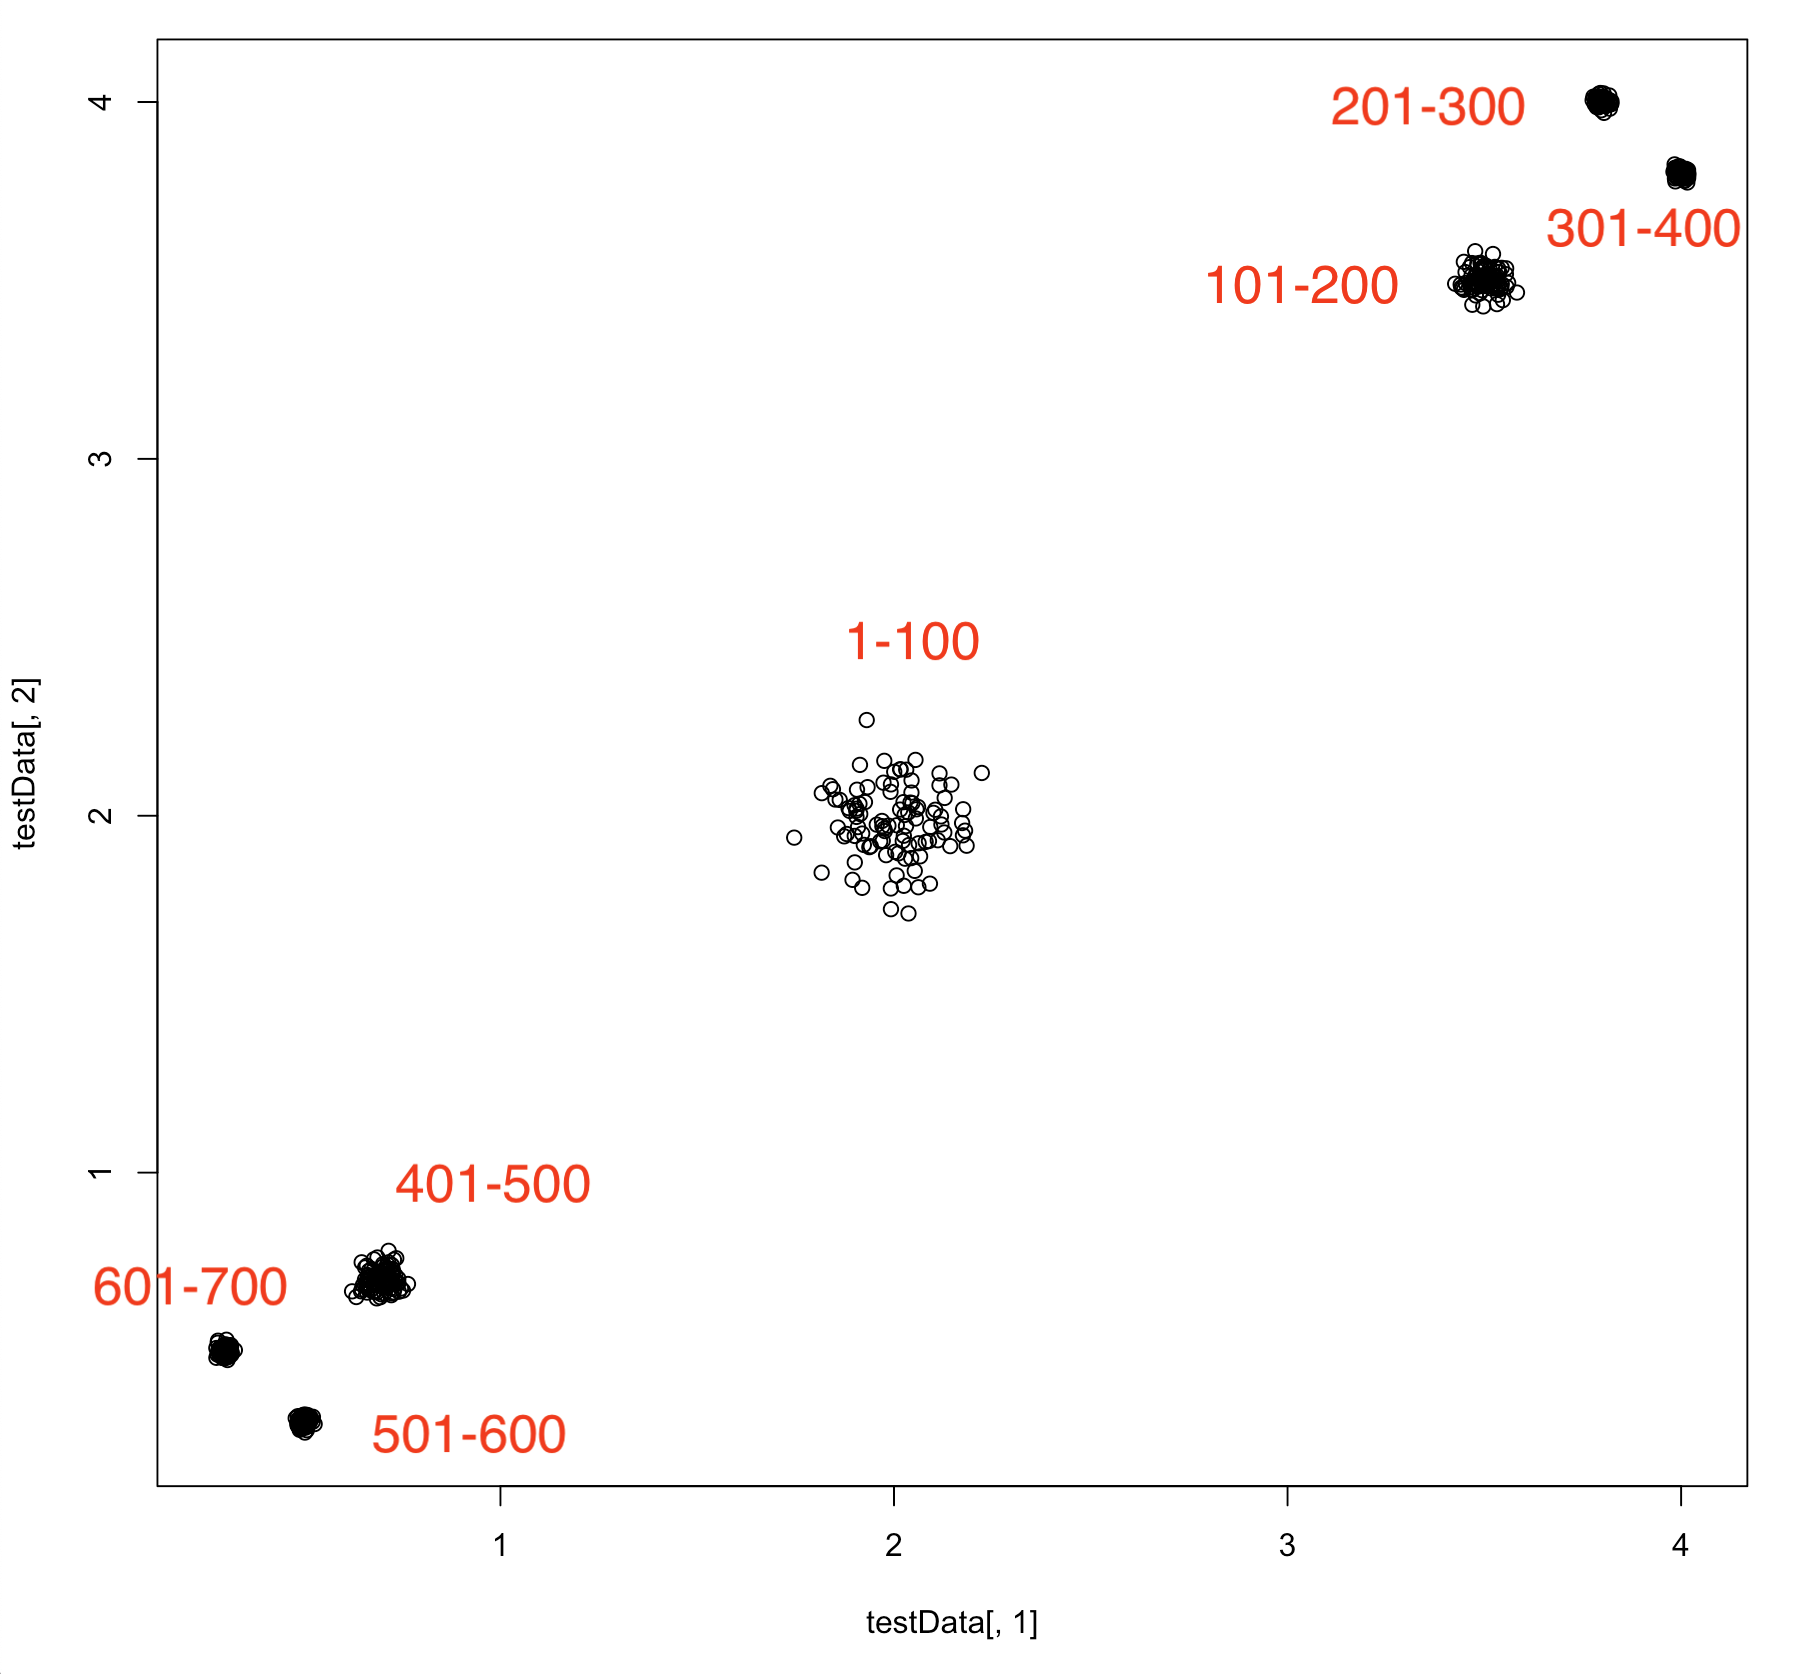
\includegraphics[scale=0.2]{figs/simulationData.png}}
	\end{itemize}
\end{frame}



\begin{frame}{Data Preprocessing}
	\begin{itemize}
		\item Simulation study 2: Three classes normal data.
		\\
		Dimension: 30,000$\times$500
		\\
		\centerline{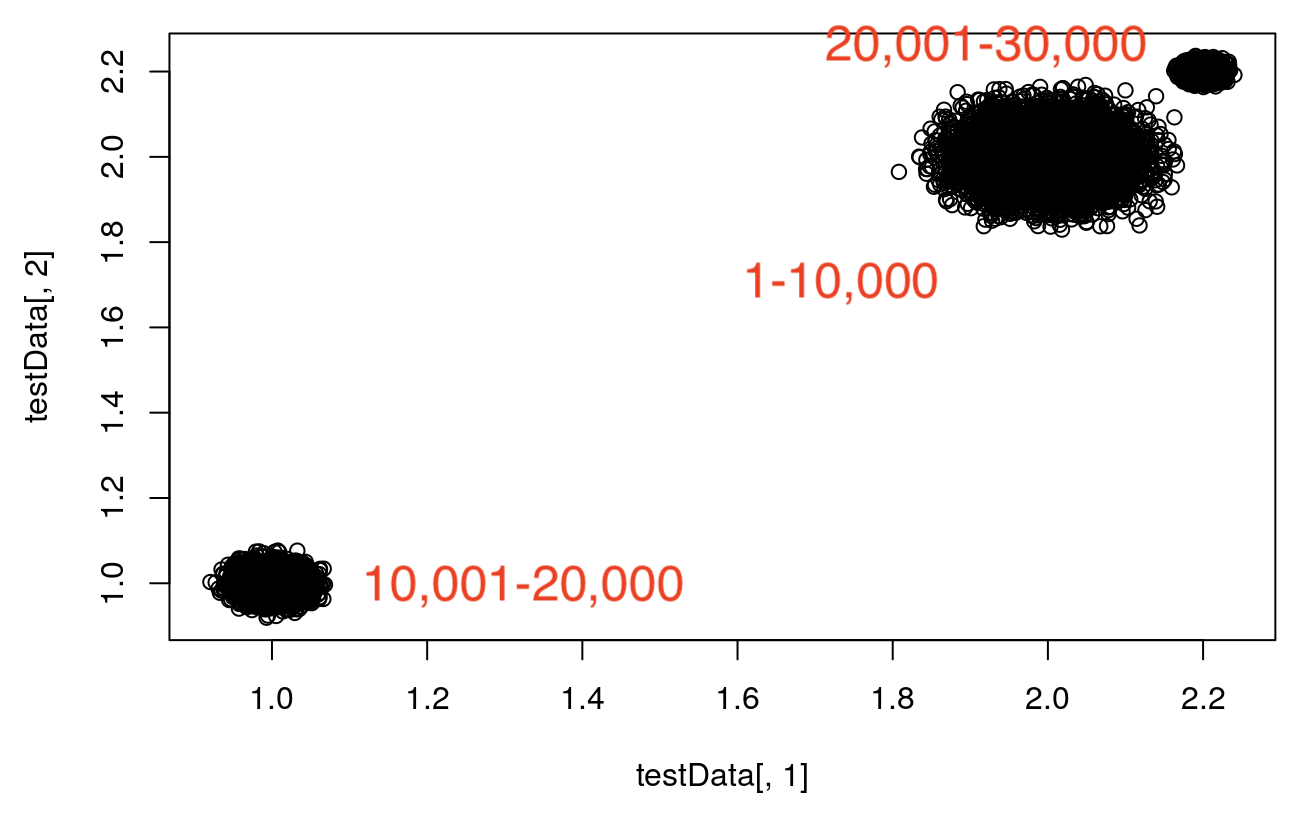
\includegraphics[scale=0.4]{figs/simulationData2.png}}
	\end{itemize}
\end{frame}



\begin{frame}{Data Preprocessing}
	\begin{itemize}
		\item Real data: MNIST		
		\\
		Dimension: 60,000$\times$154 (whole) 1,000$\times$154 (mini)
		~\\
		~\\
		\centerline{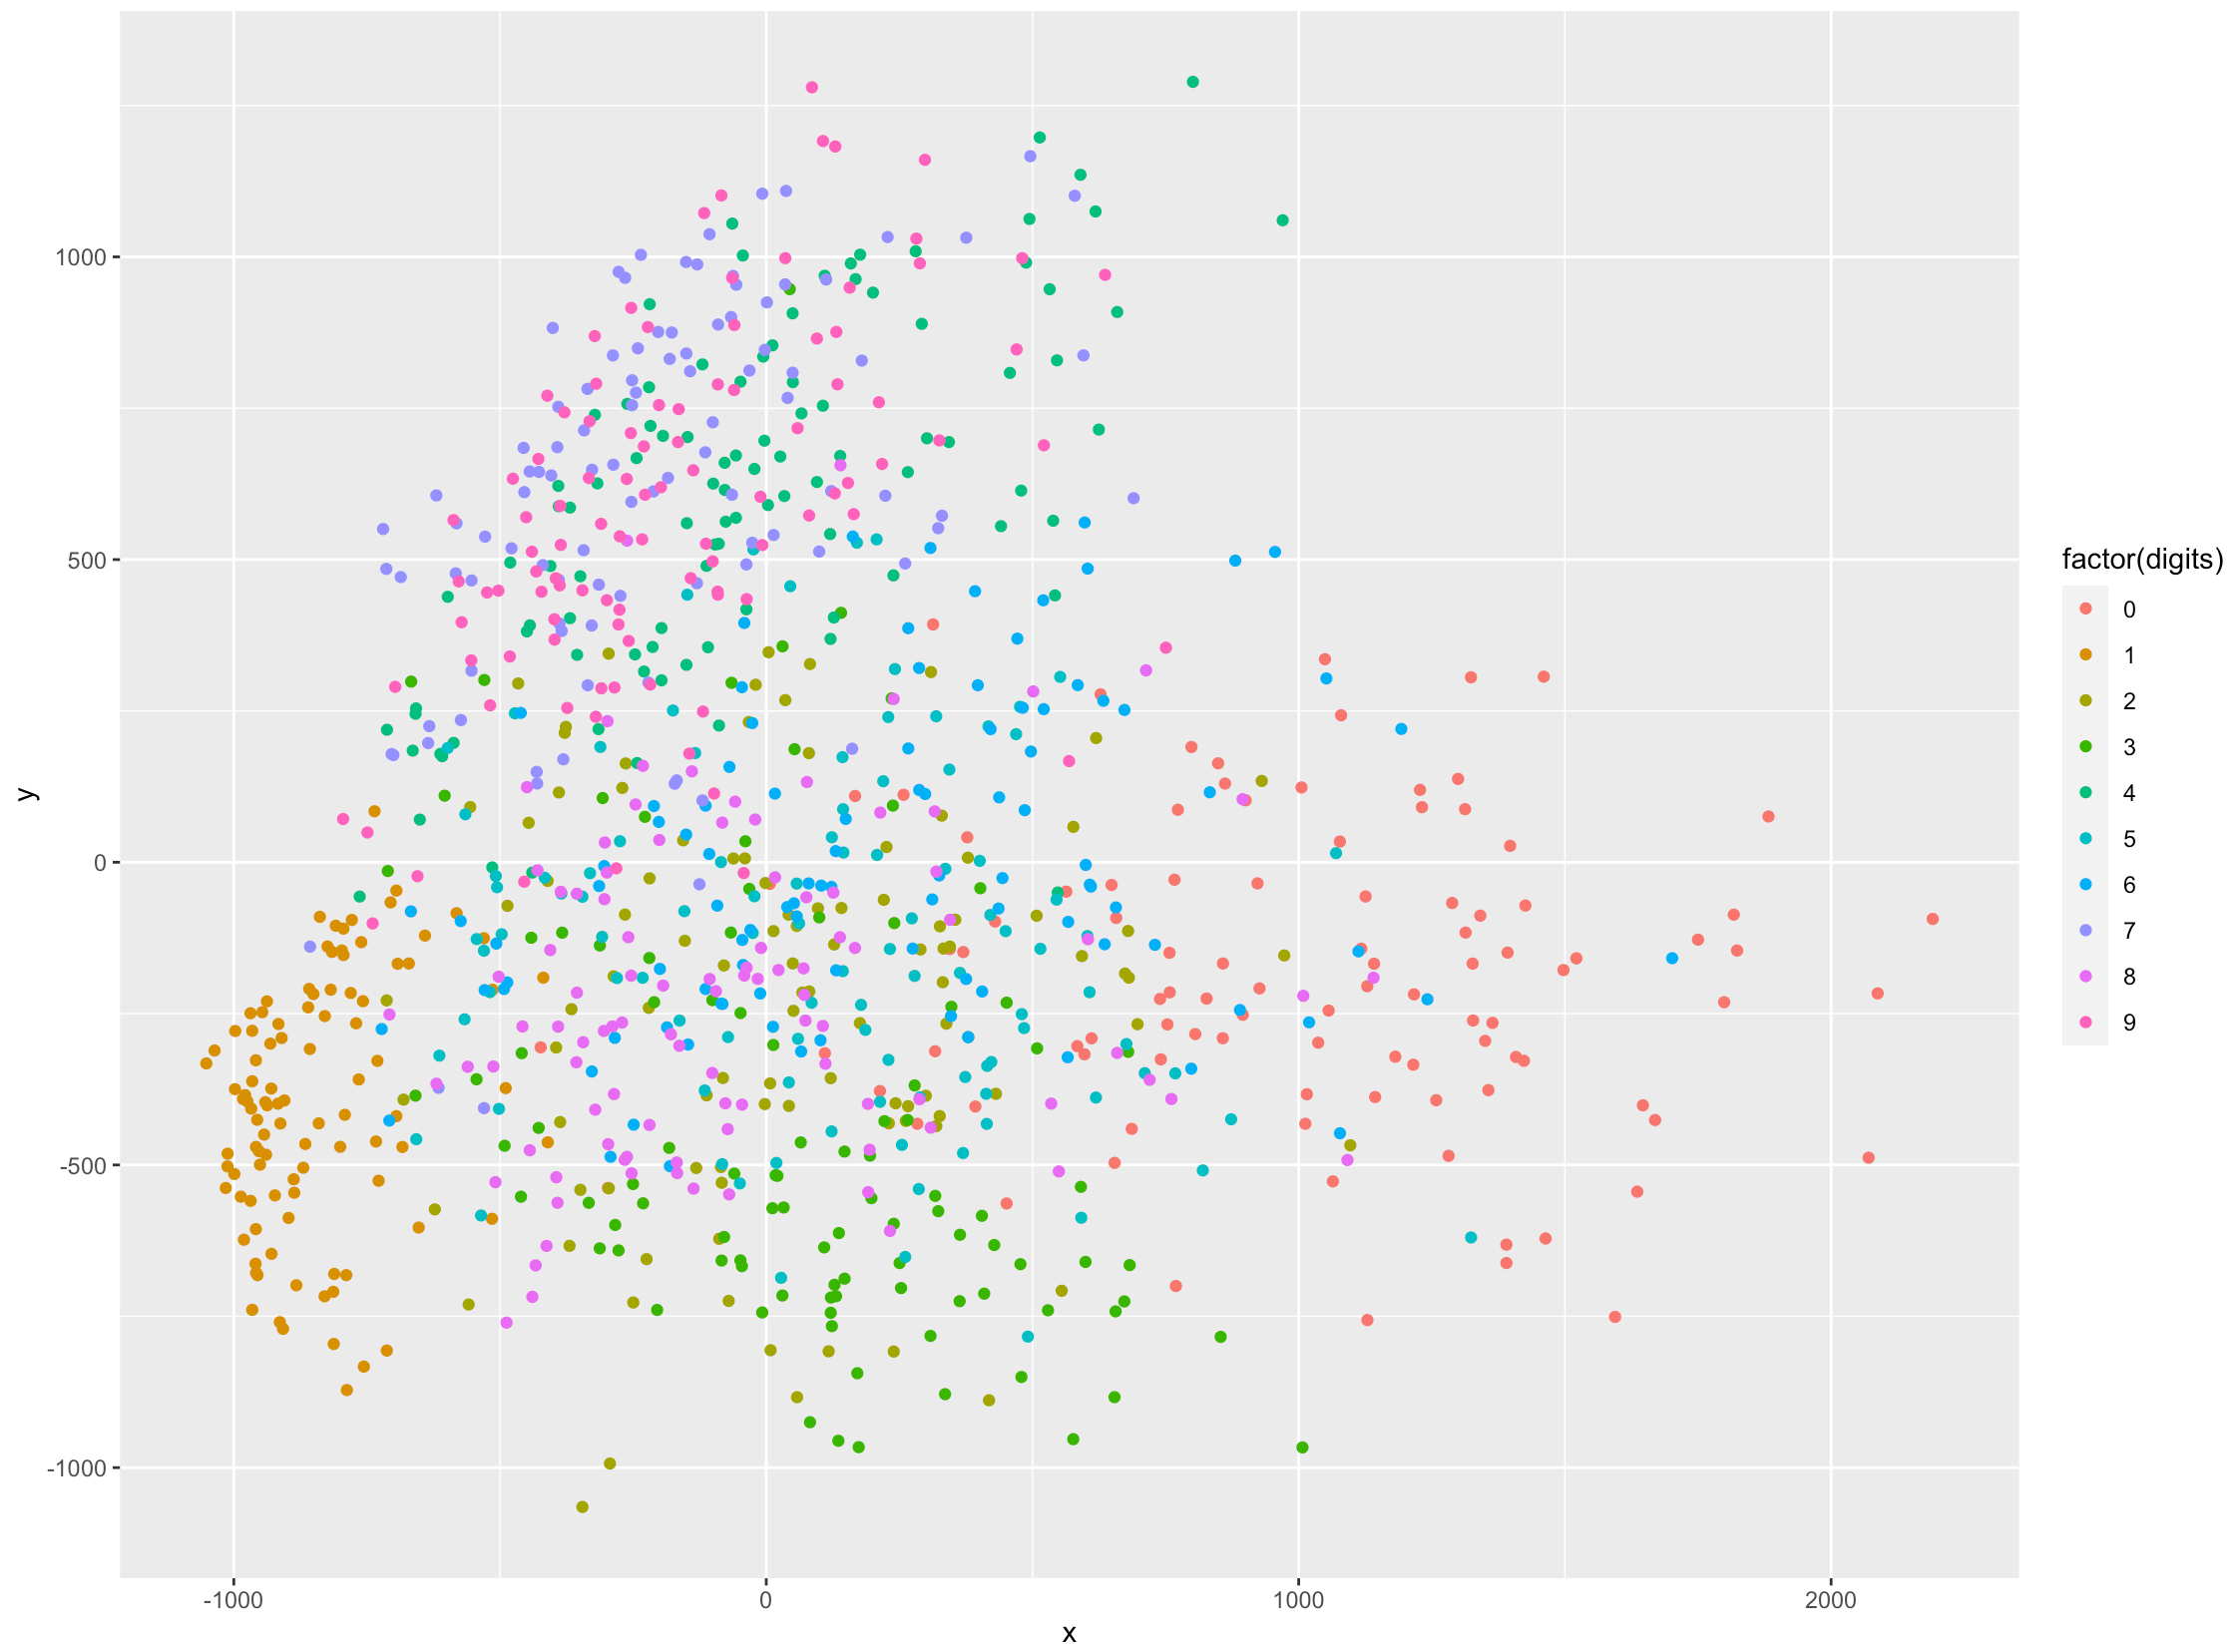
\includegraphics[scale=0.2]{figs/MNIST_mini.png}}
		miniData: 100 samples for each digit.
	\end{itemize}
\end{frame}



\begin{frame}{Preliminaries}
Dirichlet process (DP)\\
~\\
\centerline{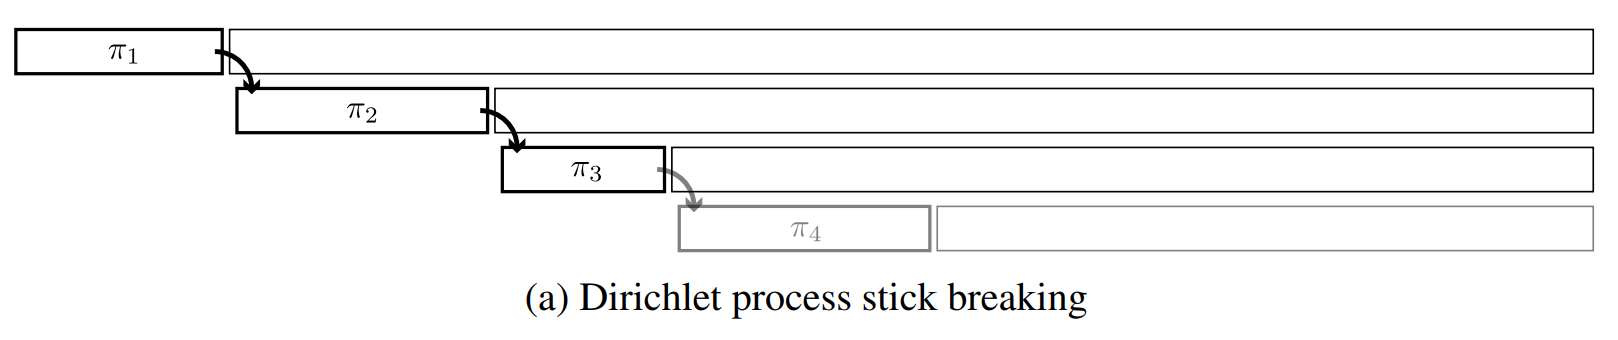
\includegraphics[scale=0.4]{figs/DP.png}}
Tree-structured stick breaking process (TSSB)\\
~\\
\centerline{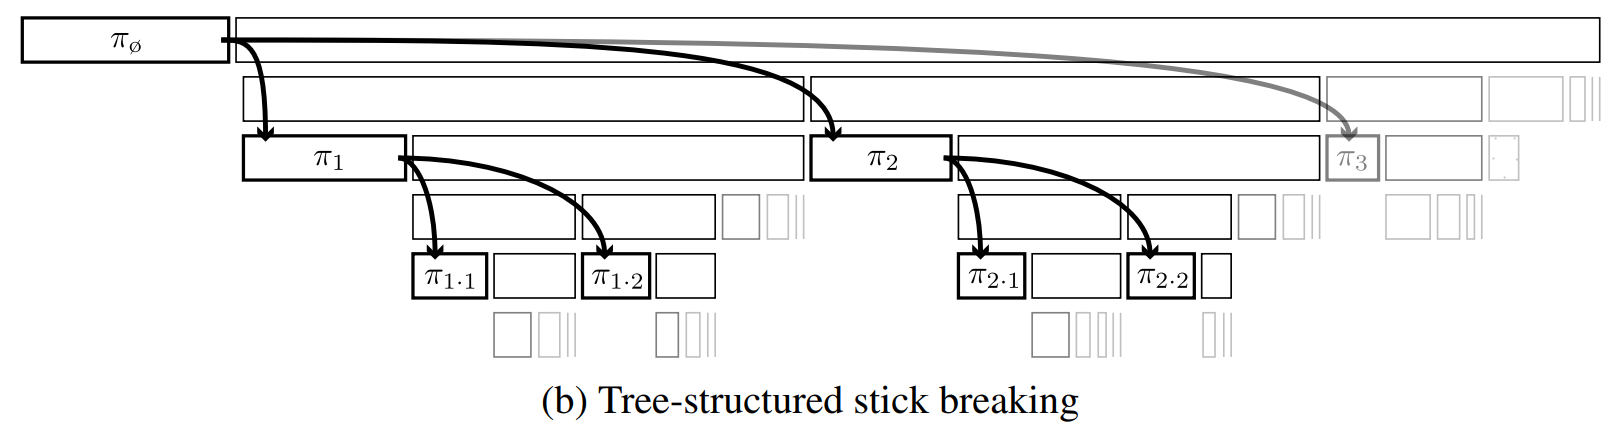
\includegraphics[scale=0.4]{figs/TSSB.png}}
\end{frame}



\begin{frame}{Our model}
Motivated by the work of Ishwaran and James (2001), our model:
~\\
~\\
\begin{itemize}
\item based on a truncation version of TSSB.
~\\
~\\
\item Use factored normal likelihood to avoid the high dimensionality problem.
~\\
~\\
\item Parameters:\\
\begin{itemize}
	\item node parameters $\theta_{\varepsilon}^\ell$ and $\sigma_{\varepsilon}^{2\ell},$ for $\ell = 1,...,L$.
	\item data assignment $c_i,$ for $i=1,...,n$.
	\item stick length $\nu$-sticks and $\psi$-sticks, which derive the random weights $\pi_\varepsilon$.
	\item hyper-parameter drift $\lambda^\ell.$ 
	\item stick-breaking hyper-parameters $\alpha_0,\lambda,\gamma$.
	\item \textbf{Fixed} parameters: $\eta_{\mathcal{N}}$ and $\eta_{\Theta}$
\end{itemize}

\item Search for new tree structure (Yuan et al.2015).\\
The authors added another swap-nodes step to propose a new tree structure.

\end{itemize}
\end{frame}

\begin{frame}{Our model}
The complete model is
$$
\begin{aligned}
\left( X_{i} \mid \theta, \Sigma, c_i=\varepsilon \right) & \stackrel{\text { ind }}{\sim} \prod_{\ell=1}^L N\left(X_{i}^\ell \mid \theta_{\varepsilon}^\ell, \eta_{\mathcal{N}}^{|\varepsilon|}\sigma_{\varepsilon}^{2\ell}\right), \quad i = 1,...,n \\
c_{i} \mid \pi & \stackrel{\text { iid }}{\sim} \sum_{\varepsilon} \pi_{\varepsilon} \delta_{{\varepsilon}} \\
\pi&\sim \text{TSSB-DW}(\alpha_0, \rho,\gamma)\\
\theta_{\varnothing}^\ell &\sim N(\theta_{\varnothing}^\ell\mid \mu_0^\ell,  \lambda^\ell), \quad \ell=1,...,L\\
\theta_{\varepsilon}^\ell \mid \theta_{pa(\varepsilon)}^\ell, \eta_{\Theta}& \stackrel{\text { iid }}{\sim} N(\theta_{\varepsilon}^\ell\mid \theta_{pa(\varepsilon)}, \eta_{\Theta}^{|\varepsilon|}\lambda^\ell)\\
\sigma_{\varepsilon}^{2\ell} &\stackrel{\text { iid }}{\sim} \text{InvGamma}(v_{sig}, s_{sig})\\
\lambda^\ell & \stackrel{\text { iid }}{\sim} \text{InvGamma}(v_{dft}, s_{dft})
\end{aligned}
$$
\end{frame}

\begin{frame}{Posterior inference}
	
\begin{itemize}
\item Resample data assignments $c_i$ for $i=1,...,n$. (multinoulli)

\item Resample node parameters $\theta_{\varepsilon}^\ell$ and $\sigma_{\varepsilon}^{2\ell}$ for $\ell = 1,...,L$. (normal-invGamma)

\item Resample stick length $\nu$-sticks and $\psi$-sticks, in order to update the random weights $\pi_\varepsilon$. (like in DP)

\item Resample hyper-parameter drift $\lambda^\ell$ for $\ell = 1,...,L$. (normal-invGamma)

\item Resample stick-breaking hyper-parameters $\alpha_0,\lambda,\gamma$ by slice sampler.
\end{itemize}

\end{frame}


\begin{frame}{Simulation Study}
\textbf{Study 1.} Seven classes normal data (low dimension).\\
~\\
\centerline{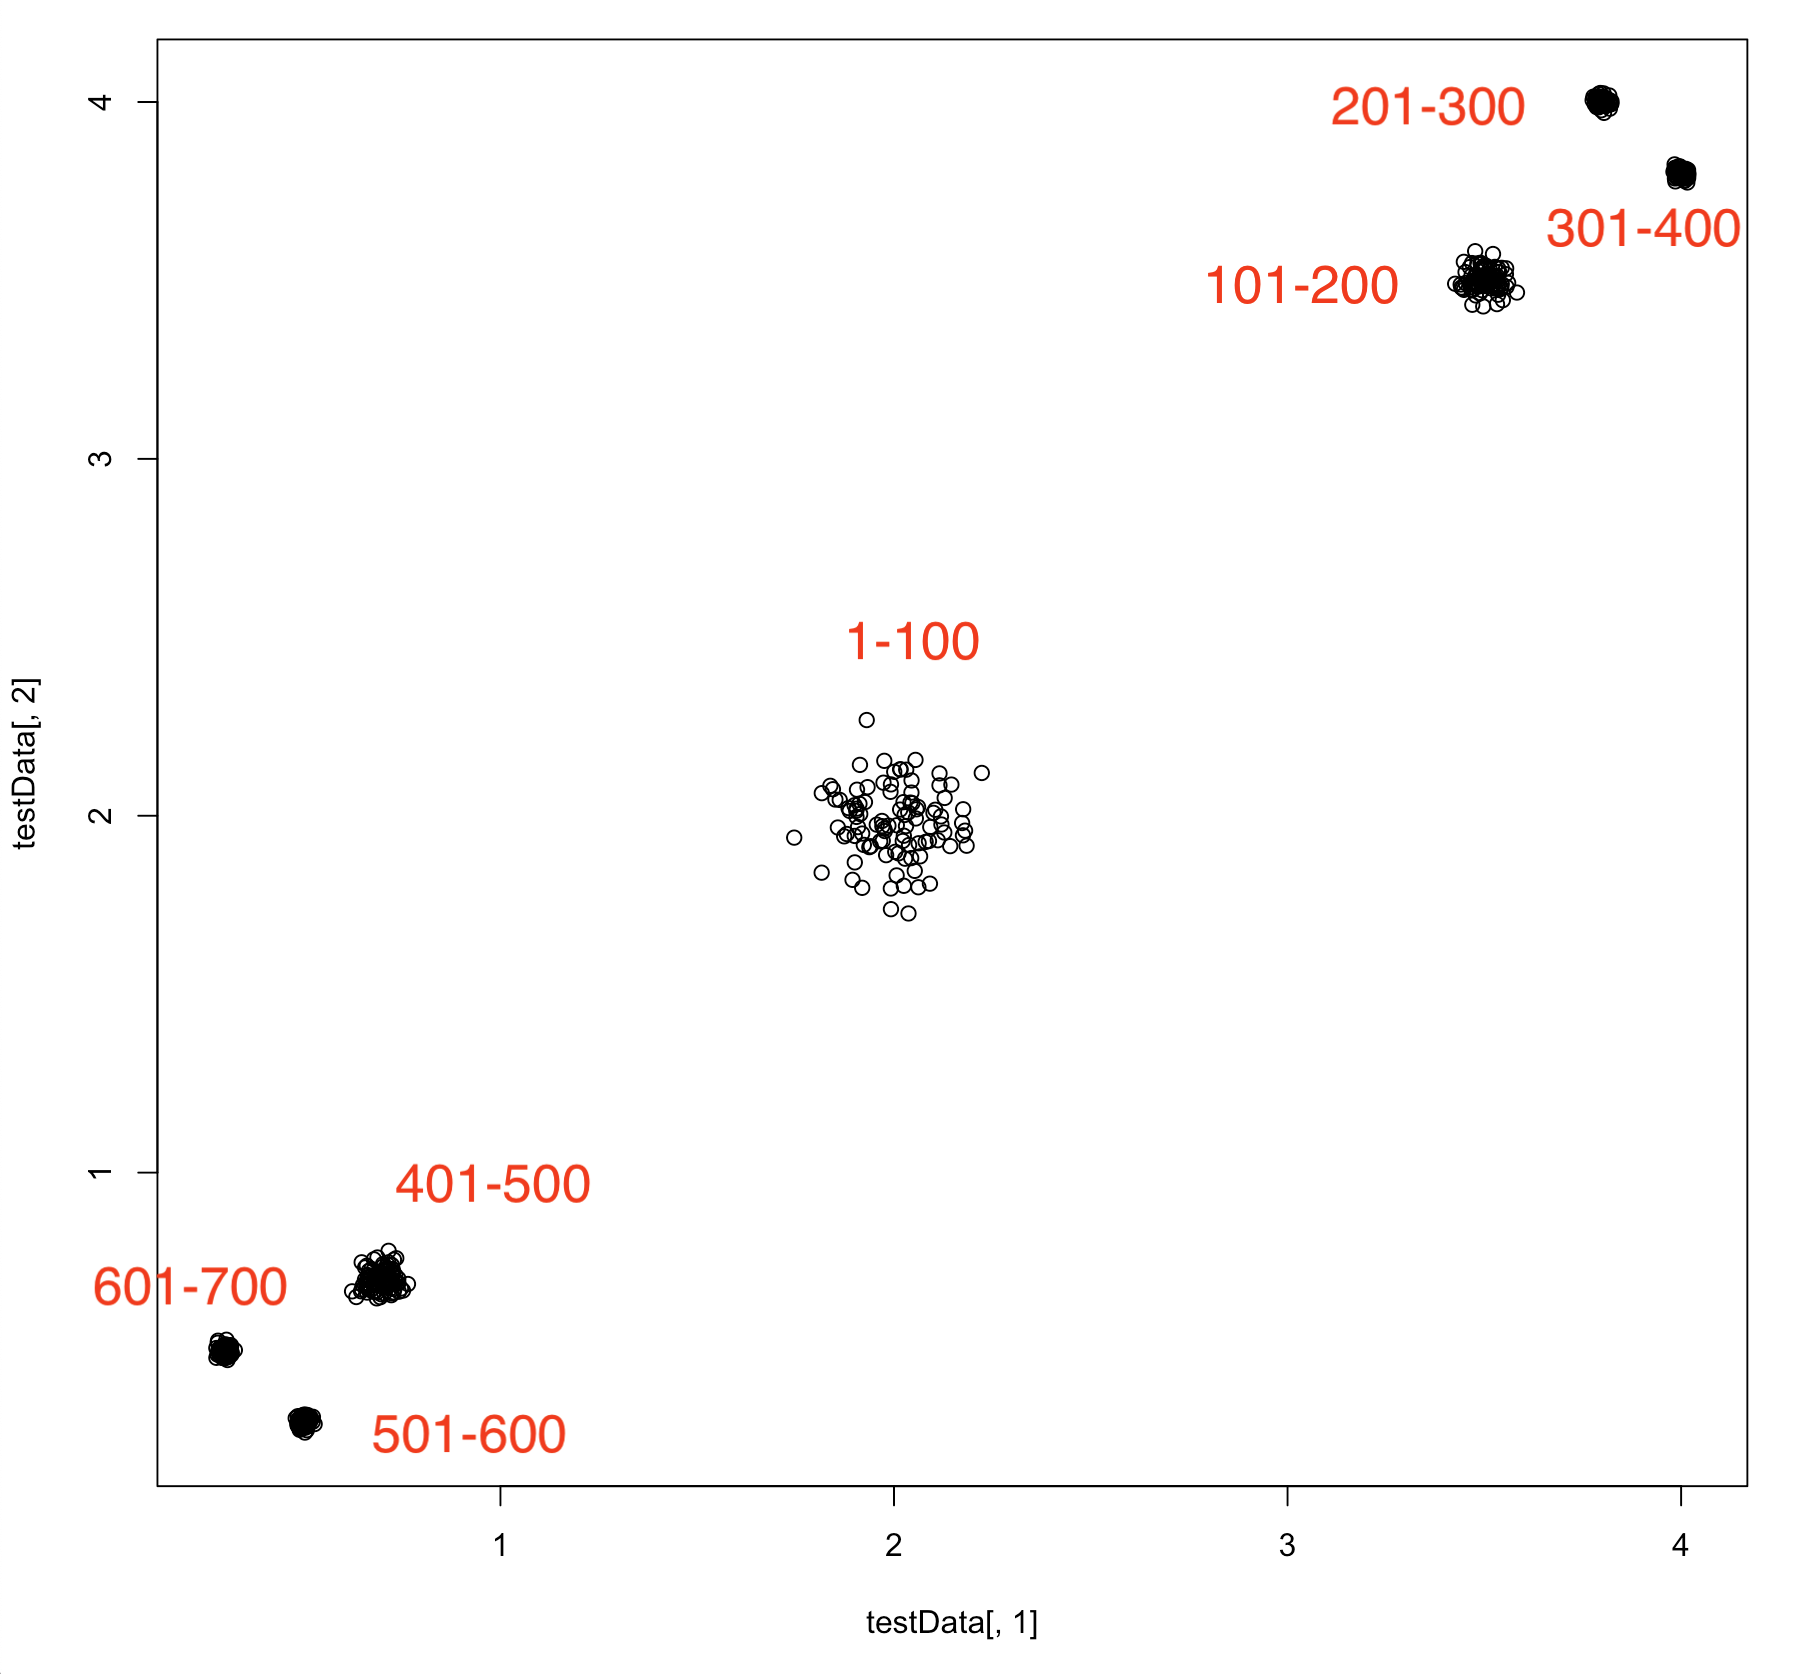
\includegraphics[scale=0.2]{figs/simulationData.png}}
\end{frame}

\begin{frame}{Simulation Study}
	Update Settings:\\
	~\\
	\begin{itemize}
		\item $\eta_{\mathcal{N}}=1$ and $\eta_{\Theta}=0.5$
		\item set.seed(9)
		\item Update order: (1) NodeParams (2) Assignments (3) SearchTree
		\item Iter = 200, burnIn = 0
		\item priorSigmaScale = mean(diag(cov(t(testData))))
		\item D = 3, W = 3
		\item "OnlyTree"
		\item $\lambda^\ell  \stackrel{\text { iid }}{\sim} \text{InvGamma}(v_{dft}, s_{dft})$
	\end{itemize}
\end{frame}


\begin{frame}{Simulation Study}
	Results\\
	~\\
\centerline{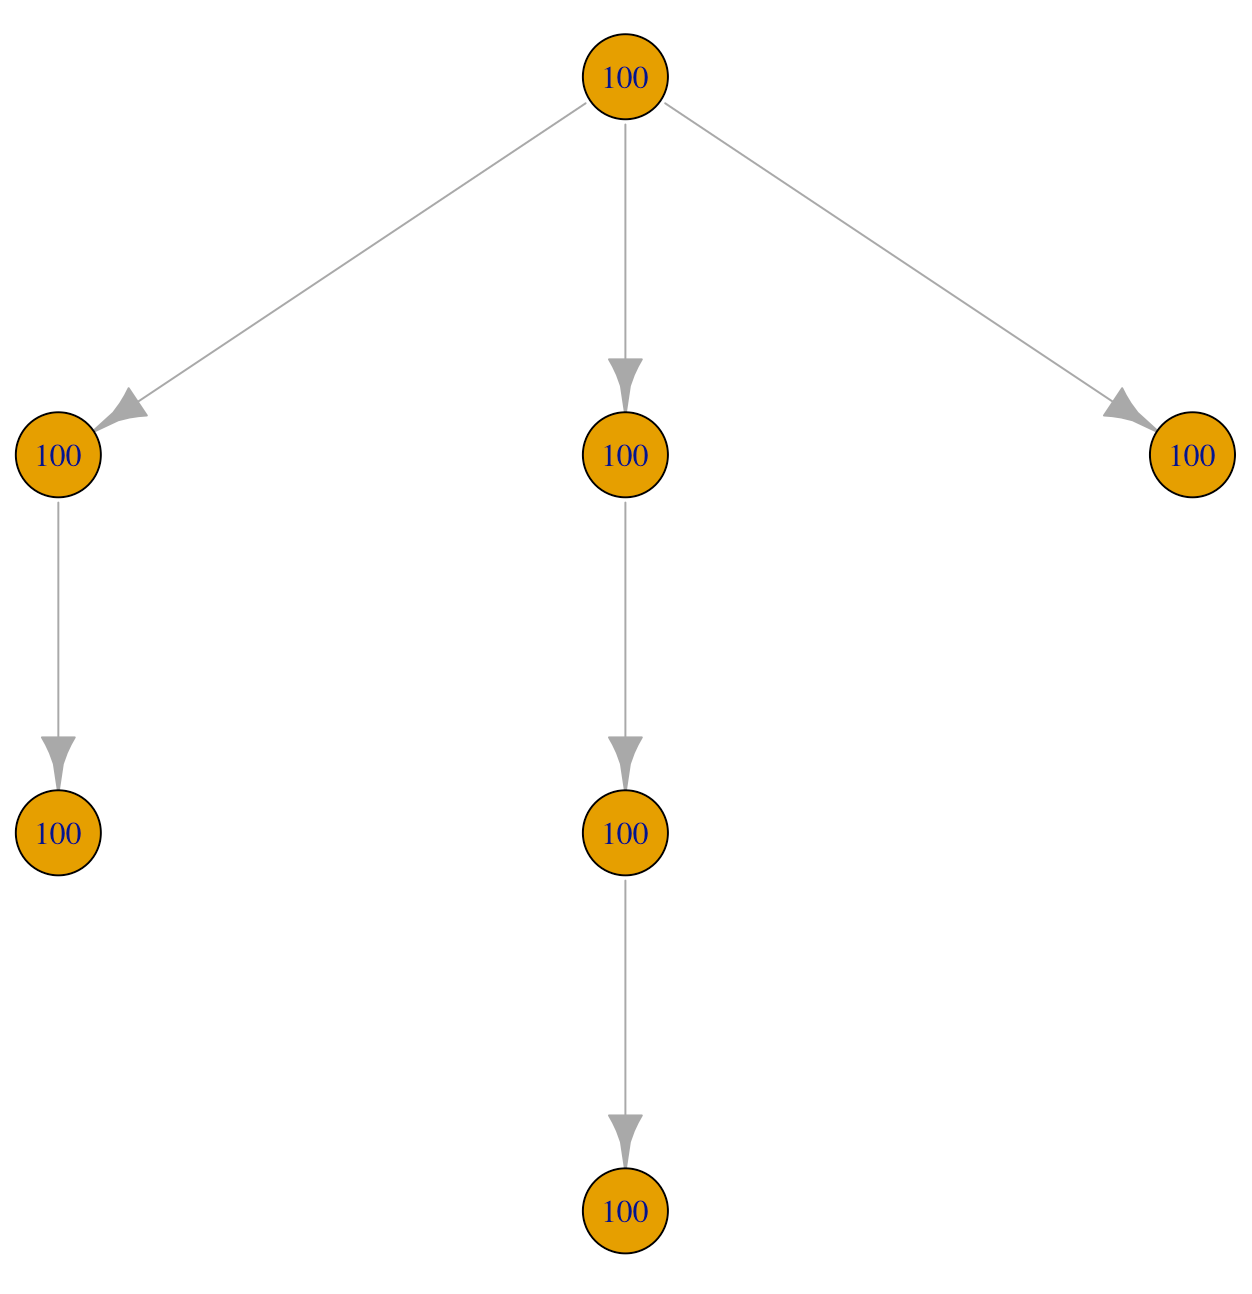
\includegraphics[scale=0.2]{figs/simRes.png}
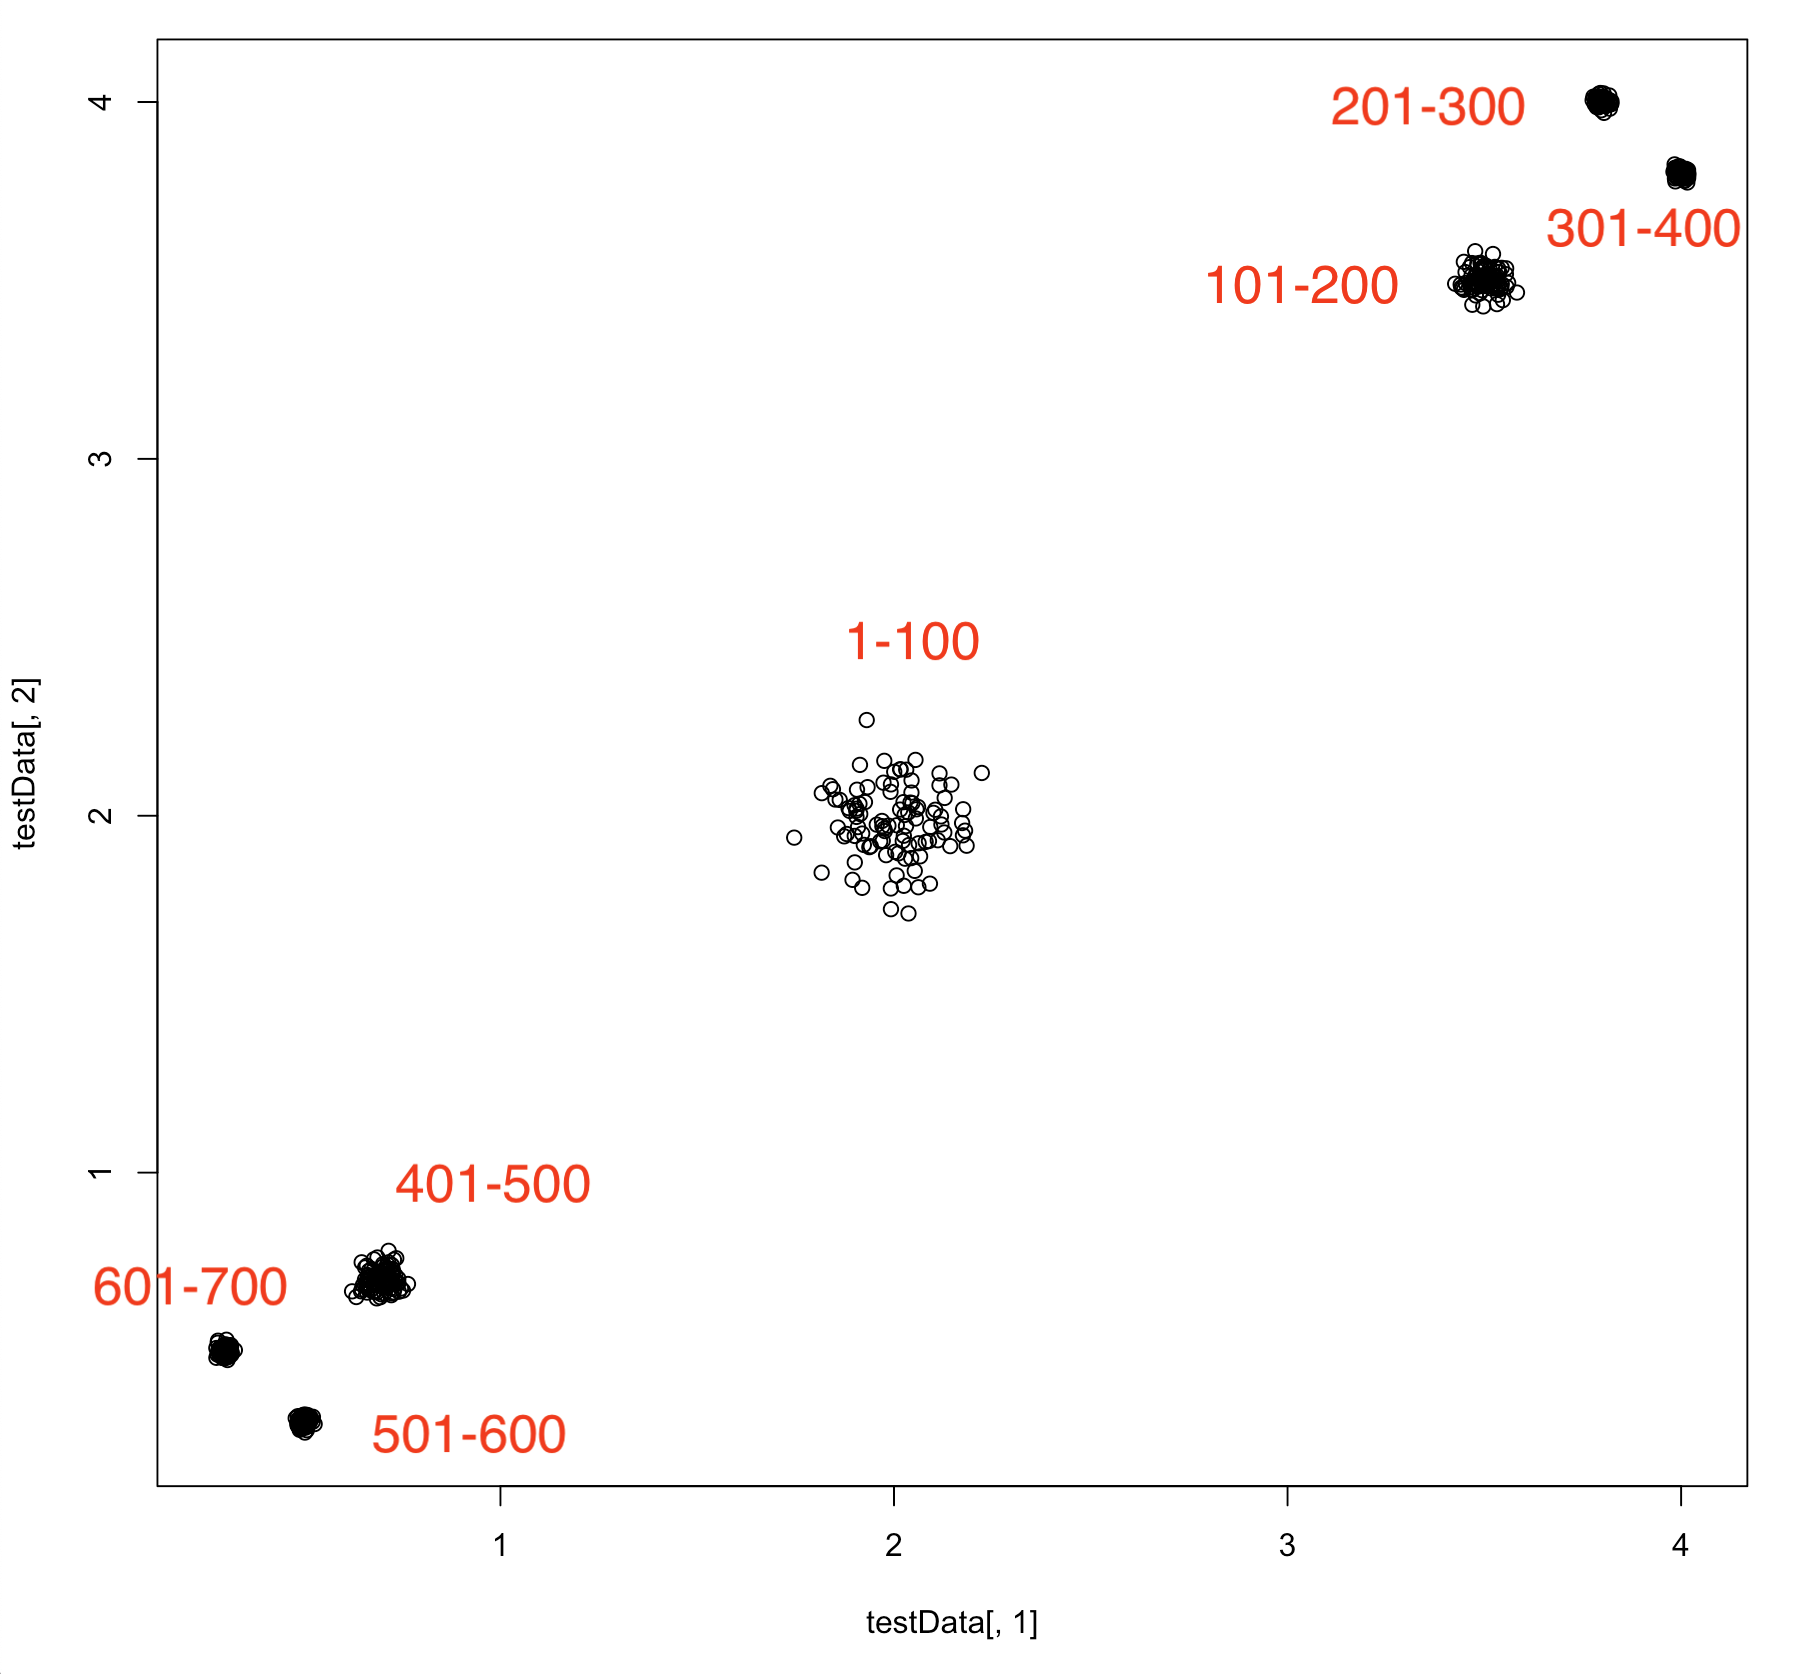
\includegraphics[scale=0.15]{figs/simulationData.png}}
~\\
Node 0 contains dataIds 401-500,  Node 1 contains dataIds 1-100  \\
Node 11 contains dataIds 501-600, Node 2 contains dataIds 301-400 \\
Node 23 contains dataIds 201-300, Node 233 contains dataIds 101-200\\
Node 3 contains dataIds 601-700.
\end{frame}



\begin{frame}{Simulation Study}
	\textbf{Study 2.} Three classes normal data (high dimension).\\
	~\\
	\centerline{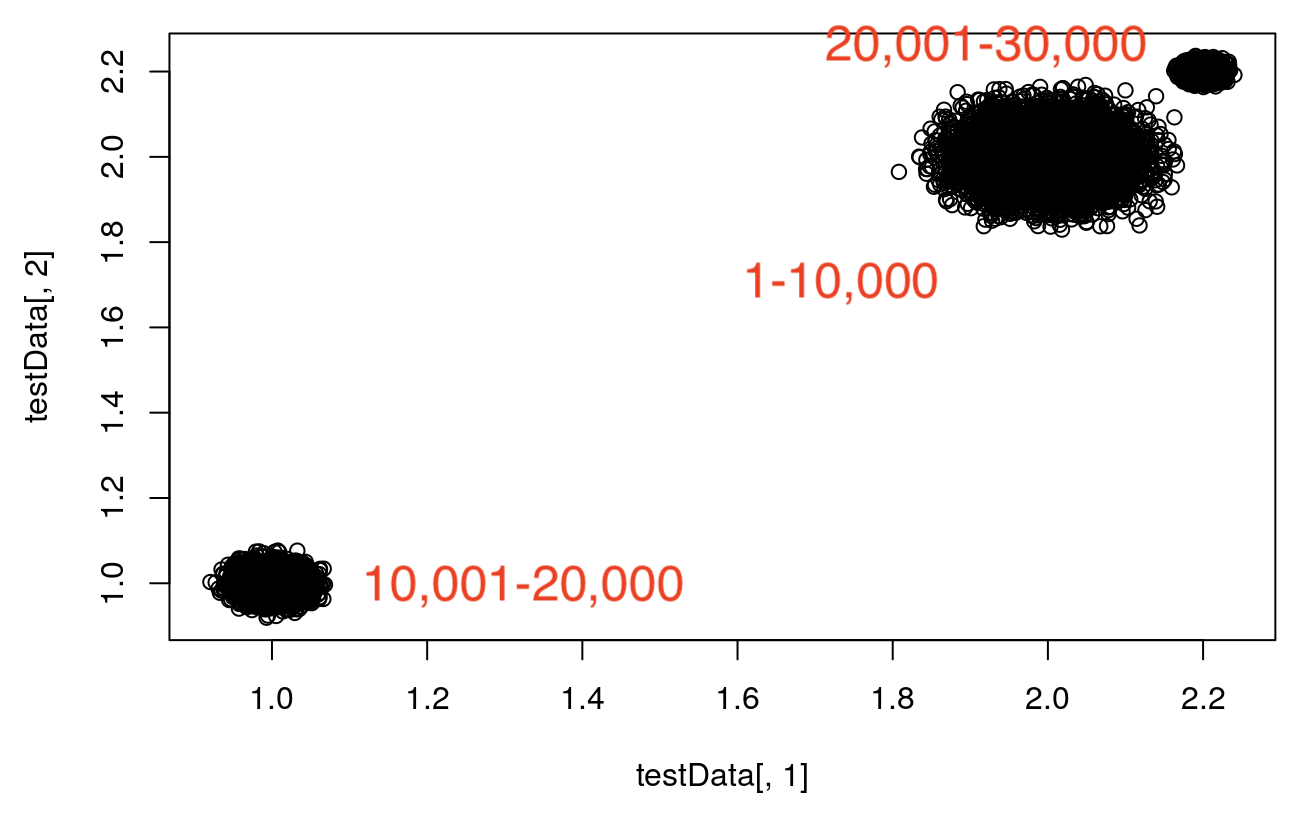
\includegraphics[scale=0.4]{figs/simulationData2.png}}
\end{frame}


\begin{frame}{Simulation Study}
	Update Settings:\\
	~\\
	\begin{itemize}
		\item $\eta_{\mathcal{N}}=1$ and $\eta_{\Theta}=1$
		\item set.seed(12)
		\item Update order: (1) NodeParams (2) Assignments \textit{(WITHOUT searchTree step)}
		\item Iter = 50, burnIn = 0
		\item priorSigmaScale = 1e-4
		\item D = 3, W = 3
		\item "OnlyTree"
		\item $\lambda^\ell  \stackrel{\text { iid }}{\sim} \text{Unif}(0.01, 1)$
	\end{itemize}
\end{frame}



\begin{frame}{Simulation Study}
	Results\\
	~\\
	\centerline{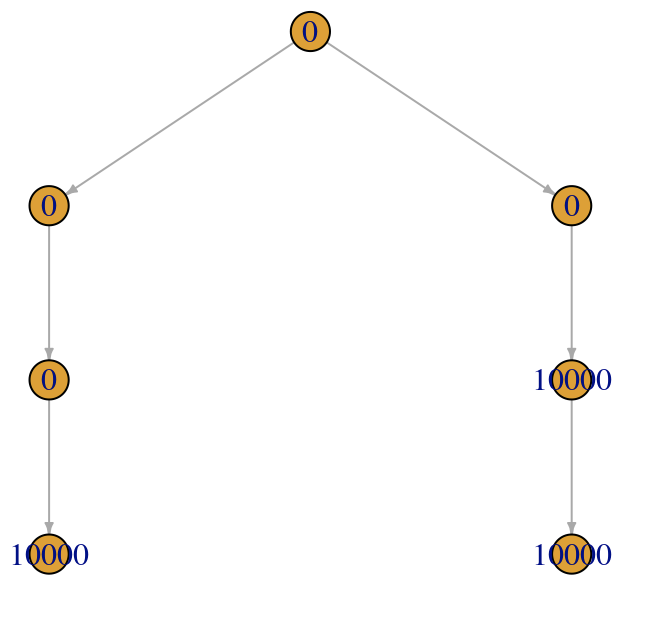
\includegraphics[scale=0.3]{figs/sim2Res.png}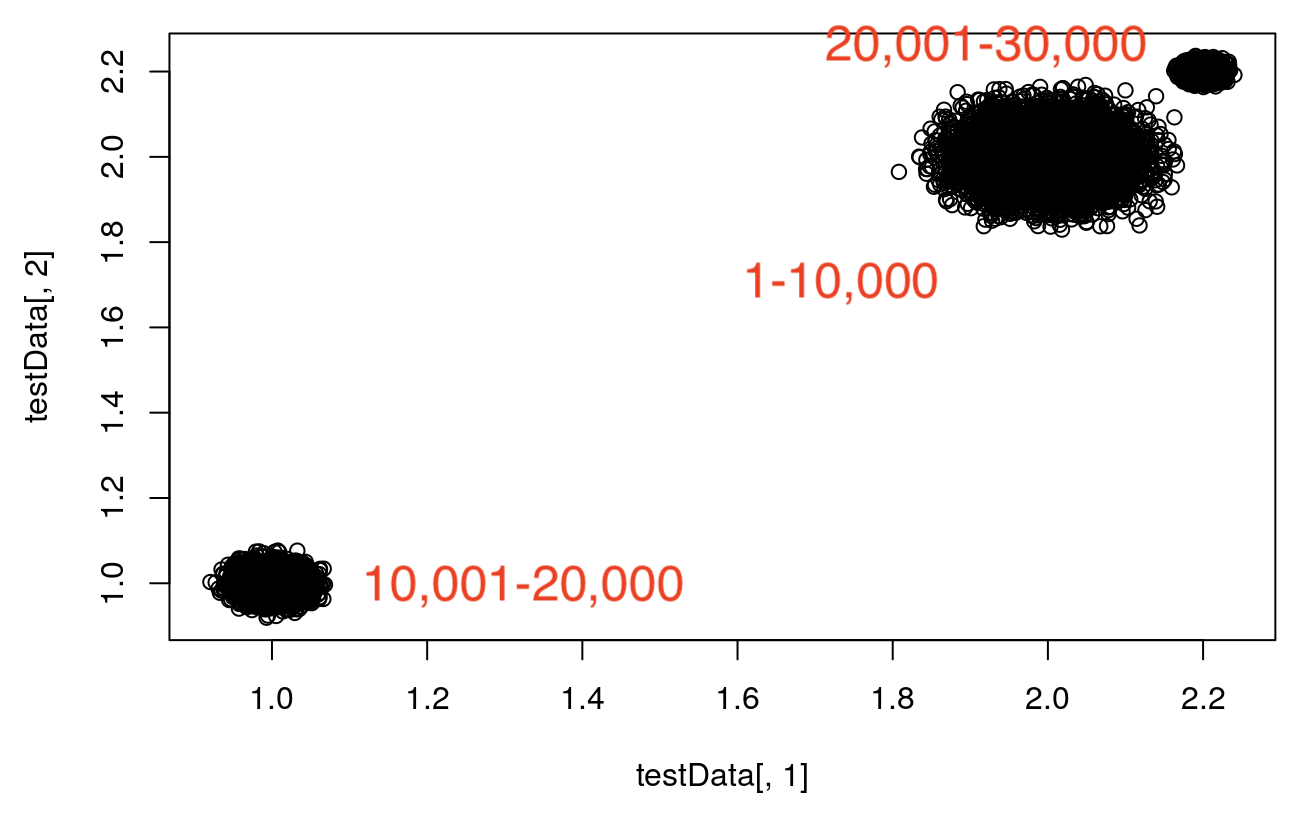
\includegraphics[scale=0.2]{figs/simulationData2.png}}
	~\\
Node 232 contains dataIds 1-10000\\
Node 33 contains dataIds 10001-20000\\ 
Node 331 contains dataIds 20001-30000
\end{frame}



\begin{frame}{MNIST}
MNIST: A famous handwritten digits dataset. It includes a training set with 60,000 images and a test set with 10,000 images. Each image has 28x28 pixels. Each pixel in the image matrix is in [0,255].\\
~\\
	\centerline{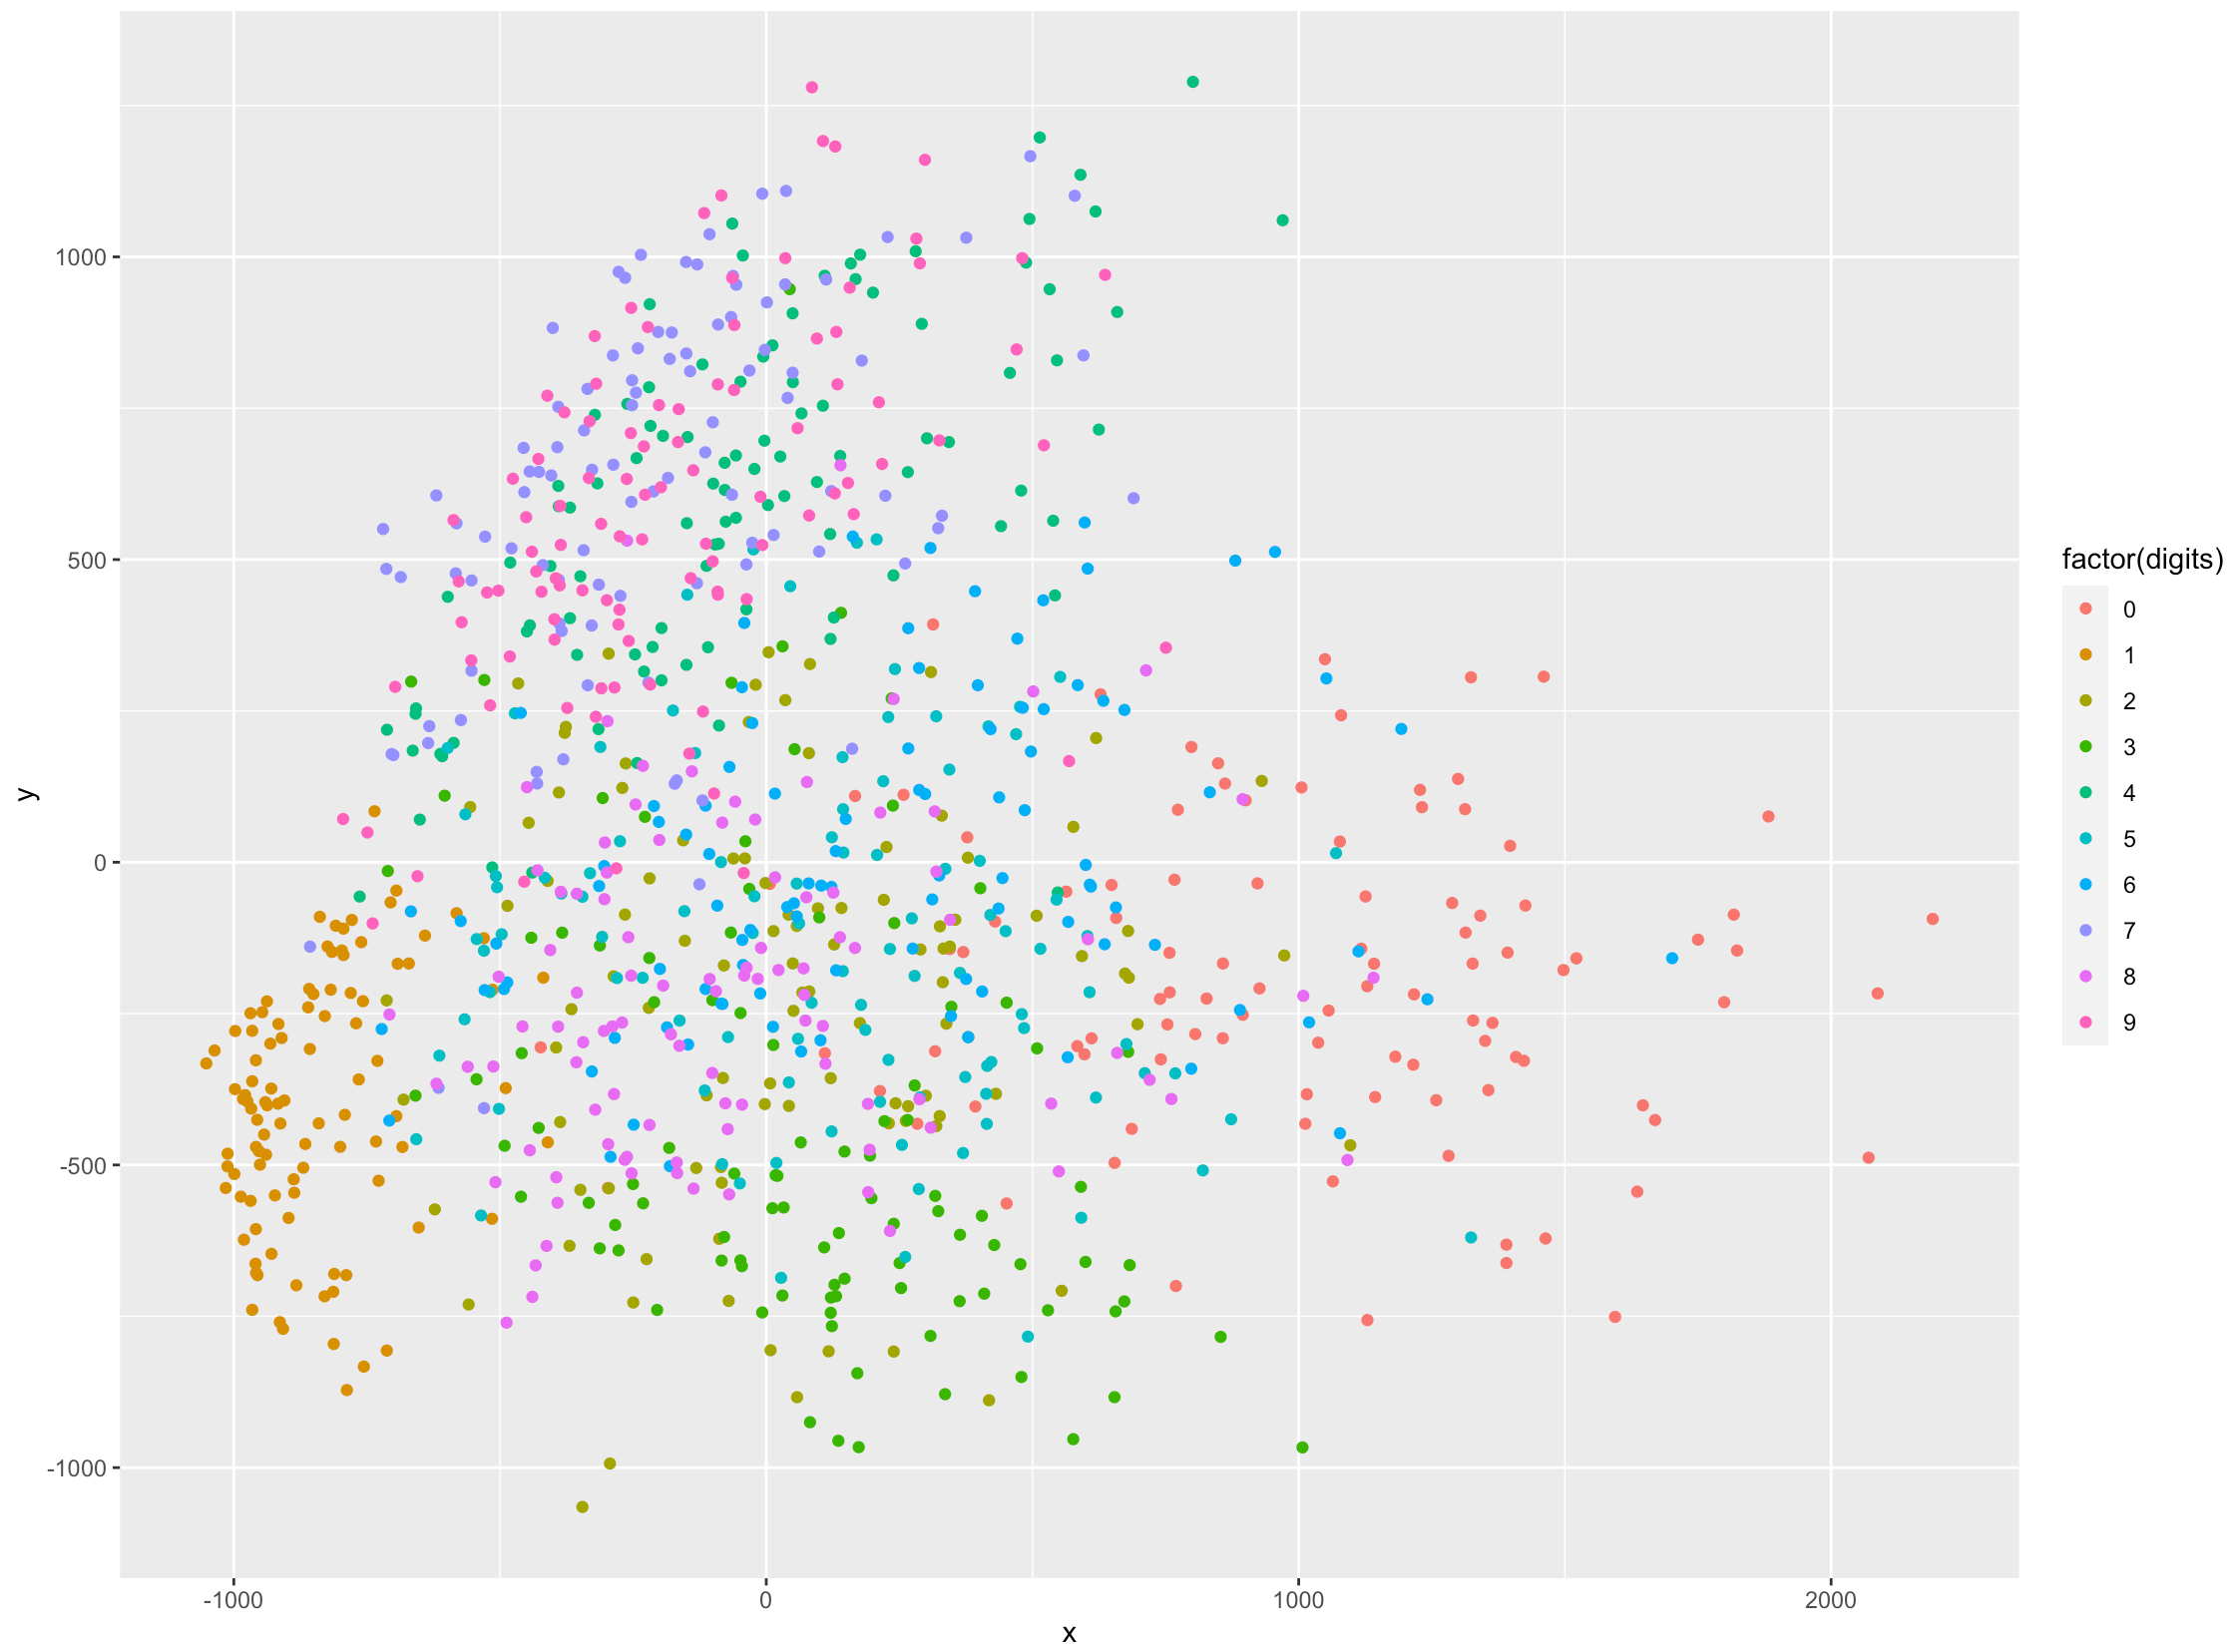
\includegraphics[scale=0.2]{figs/MNIST_mini.png}}
	~\\
\end{frame}



\begin{frame}{MNIST}
	Results under same settings.\\
	~\\
	\centerline{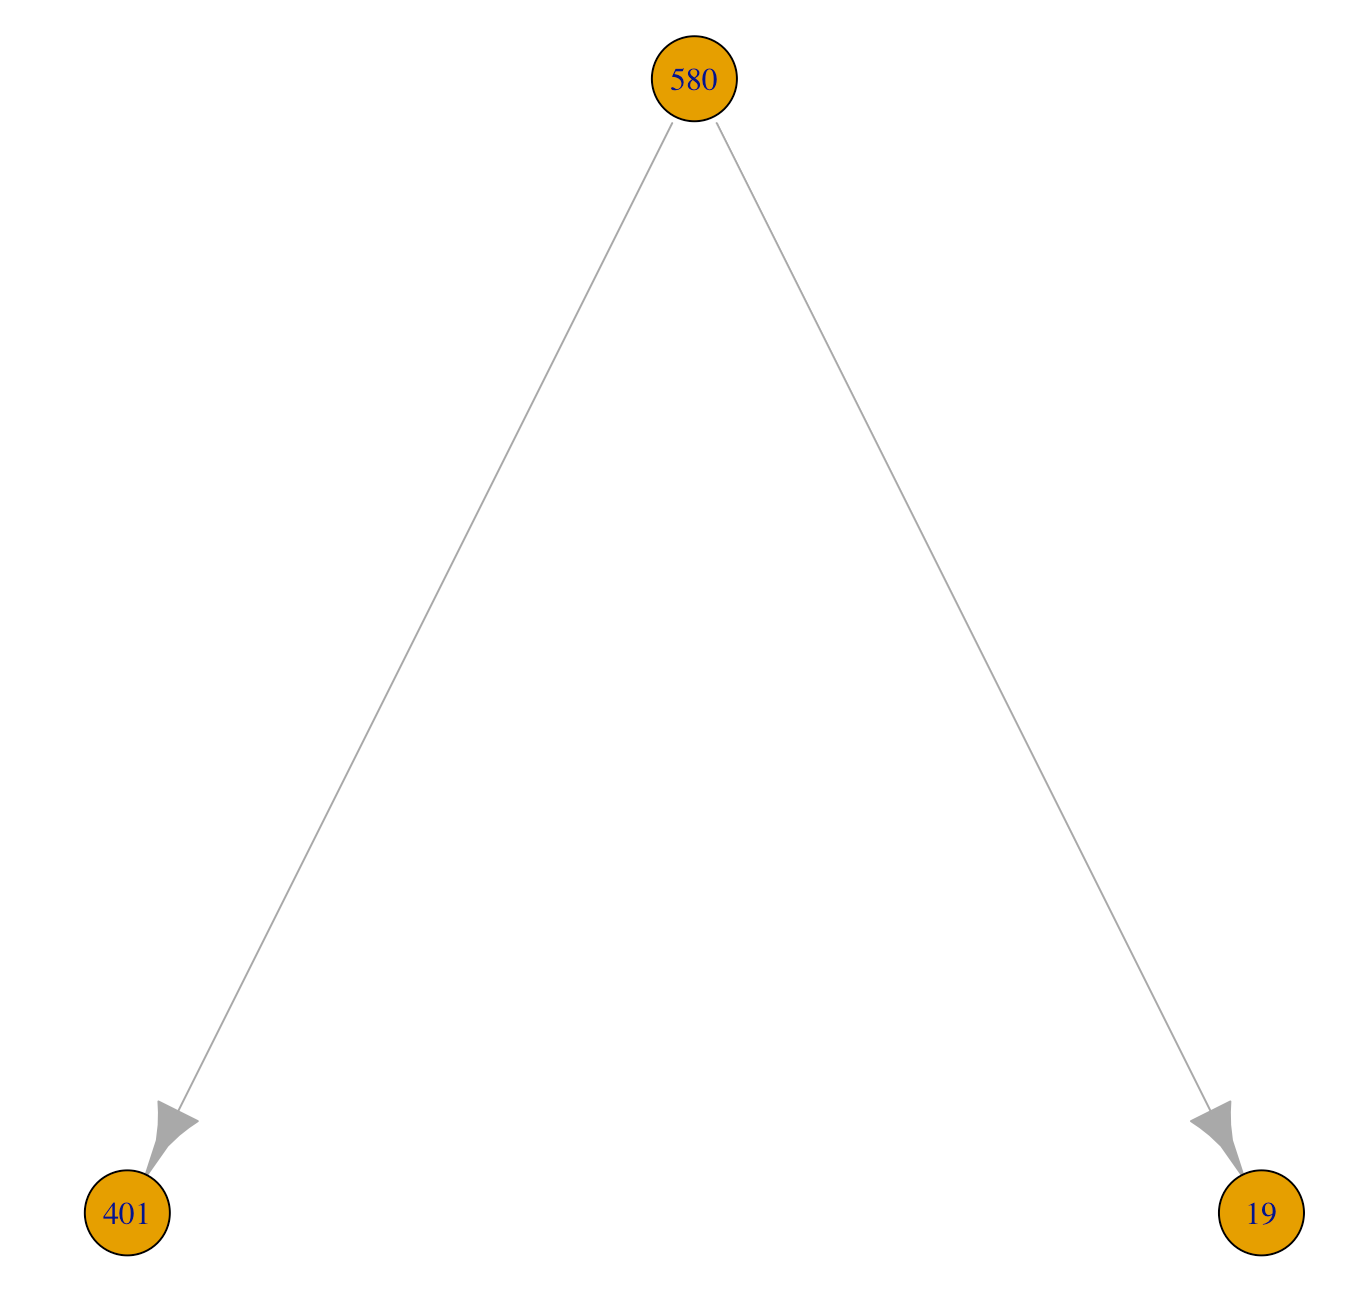
\includegraphics[scale=0.15]{figs/mnistRes.png}}
	~\\
    Root: 0 ( 53 ), 1 ( 0 ), 2 ( 92 ), 3 ( 62 ), 4 ( 64 ), 5 ( 77 ), 6 ( 63 ), 7 ( 45 ), 8 ( 84 ), 9 ( 40 )\\
    
    Child One: 0 ( 46 ), 1 ( 100 ), 2 ( 6 ), 3 ( 36 ), 4 ( 36 ), 5 ( 17 ), 6 ( 36 ), 7 ( 55 ), 8 ( 12 ), 9 ( 57 \\
    
    Child Two: 0 ( 1 ), 1 ( 0 ), 2 ( 2 ), 3 ( 2 ), 4 ( 0 ), 5 ( 6 ), 6 ( 1 ), 7 ( 0 ), 8 ( 4 ), 9 ( 3 )
\end{frame}







\begin{frame}{Conclusion}
\begin{itemize}
	\item TSSB-DW model works well when the data are separable.
	~\\
	~\\
	\item MCMC approach obtains samples from the joint posterior distribution, so it is possible to derive a tree structure different from the original setting.
	~\\
	~\\
	\item MNIST may not be a good example for tree-structured clustering. Most digital samples overlap and the variances of each class have no obvious difference.
\end{itemize}
\end{frame}

\begin{frame}{Future Work}
\begin{itemize}
	\item Try more simulation studies.
		~\\
	~\\
	\item Try to solve the inseparable data clustering problem.
		~\\
	~\\
	\item Find a better way to choose the tree structure from all the samples and interpret the result.
	\end{itemize}
\end{frame}

\end{document}